\subsection{Chia tập huấn luyện, kiểm định và kiểm tra}
\label{subsec:4_2_2}
Hai tệp nguồn được giữ đúng vai trò ban đầu. Tệp \texttt{adult.data} là dữ liệu phát triển và được chia tiếp thành train và validation; \texttt{adult.test} được dành cho đánh giá cuối. Bước chia tập không điền thiếu, mã hóa, chuẩn hóa hoặc loại mẫu.

Các dòng có cùng toàn bộ 14 thuộc tính đầu vào được gán cùng một nhóm, trong đó giá trị thiếu được biểu diễn nhất quán. Nhãn \texttt{income} không nằm trong khóa nhóm. Cách chia dùng \texttt{StratifiedGroupKFold} với năm fold, bật trộn nhóm, seed 42 và lấy cố định fold số 0 làm validation~\cite{sklearn-sgkf}. Bốn fold còn lại làm train. Đây là một lần chia đã định trước, không lựa chọn fold hoặc seed theo điểm mô hình. Tỷ lệ số dòng chỉ xấp xỉ 80/20 vì nhóm được giữ nguyên.

\begin{table}[htbp]
\centering\small
\caption{Phân chia dữ liệu đã khóa ở bước 3}\label{tab:split-stage3}
\begin{tabular}{lrrp{.32\textwidth}}
\toprule
Tập & Số mẫu & Tỷ lệ trong development & Vai trò \\
\midrule
Train & 26.049 & 80,00\% & Fit tiền xử lý và huấn luyện \\
Validation & 6.512 & 20,00\% & Đối chiếu cấu hình đã chọn \\
Test UCI & 16.281 & --- & Đánh giá cuối \\
\bottomrule
\end{tabular}
\end{table}

Tỷ lệ lớp \texttt{>50K} là 24,08\% trong train và 24,08\% trong validation, chênh lệch 0,0029 điểm phần trăm. Phần kiểm tra này chỉ mô tả train và validation, không lập phân phối nhãn test.

\begin{figure}[htbp]
\centering
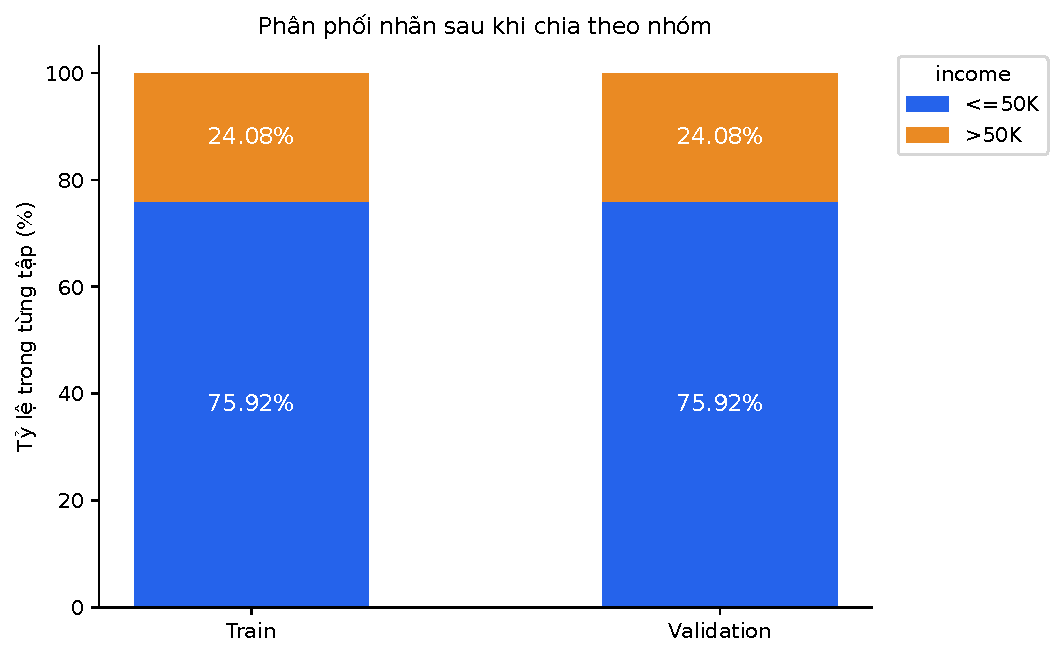
\includegraphics[width=.85\textwidth]{Images/chapter_4/4_2/4_2_2/train_validation_balance.pdf}
\caption{Phân phối nhãn của train và validation sau khi chia theo nhóm}
\label{fig:split-balance}
\end{figure}

Hai tập được xuất dưới dạng CSV cùng các tệp metadata chứa tệp nguồn, chỉ số dòng gốc và mã nhóm. Các chỉ số train/validation được khóa trong \texttt{results/step\_03/split\_indices.json}, kèm dấu vân tay của dữ liệu phát triển và phiên bản thư viện tạo split. Notebook nhúng manifest này để tái dùng chính xác tập chia giữa các môi trường; trước khi tái dùng, chương trình kiểm tra lại dữ liệu và cấu hình. Thứ tự dòng trong mỗi tập theo thứ tự nguồn.
